\subsection{Results Test Runs} % (fold)
\label{sub:results_test_runs}
This section tests that the results screen works correctly.

\subsubsection{Connects to State Store} % (fold)
\label{ssub:connects_to_state_store}
This test ensures that the component can connect to the state store.
\begin{figure}[h!]
  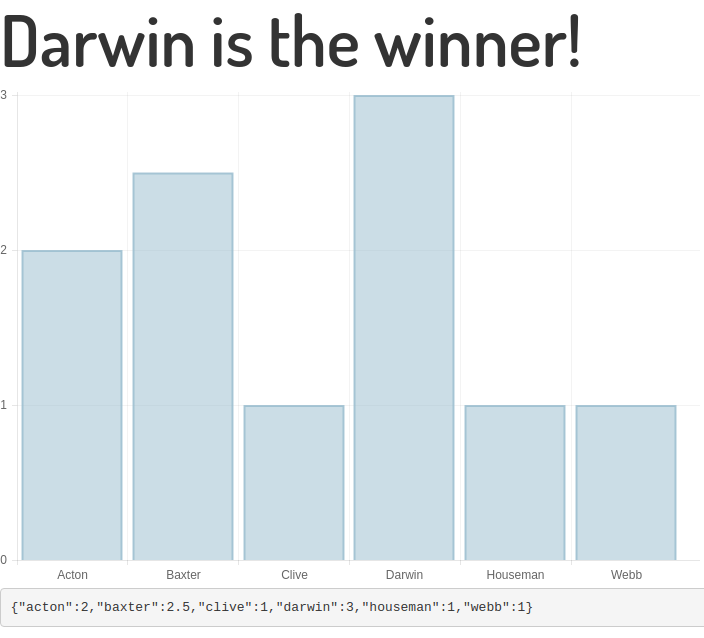
\includegraphics[scale=0.35]{testing/connect/results}
  \caption{Props view of ResultsContainer, showing the state store being passed.}
\end{figure}
As the screenshot demonstrates, the state has been passed to the component correctly, meaning the connection succeeded. \textit{Success.}
% subsubsection connects_to_state_store (end)

\clearpage

\subsubsection{Display Correct Results} % (fold)
\label{ssub:display_correct_results}
This test ensures that the results screen shows the correct results.
\begin{figure}[!htbp]
\centering
\begin{subfigure}{0.5\textwidth}
  \centering
  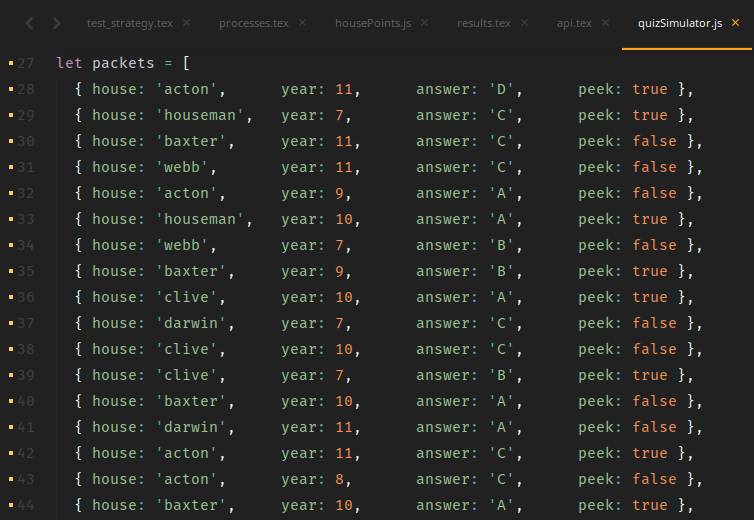
\includegraphics[width=0.95\linewidth]{testing/results/editor}
  \caption{Adding the packets to the simulation program.}
  \label{fig:sub1}
\end{subfigure}%
\begin{subfigure}{0.5\textwidth}
  \centering
  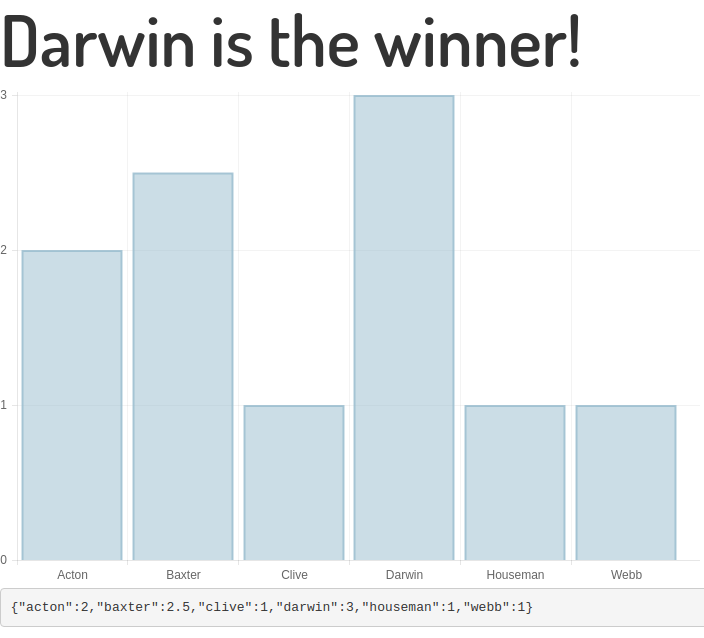
\includegraphics[width=0.95\linewidth]{testing/results/chart}
  \caption{The results chart displayed after the quiz.}
  \label{fig:sub2}
\end{subfigure}
\caption{Displaying the correct results.}
\label{fig:test}
\end{figure}
\\As can be seen, the winner and the values reflected in the chart match those in the test plan, meaning the system shows the correct results. \textit{Success.}
% subsubsection display_correct_results (end)
% subsection results_test_runs (end)
